\chapter{Conclusion and Future Work}
\label{conclusion}

\color{red}
\section{Current Prototype's Limitations and Possible Design Changes}

\section{Utilizing Locomotion Controllers to Enable High Level Trajectory Planning}


\color{blue}
TODO: Most of the text below will be moved to other sections or deleted 

\section{\SB{} Current State}
At this point, the first goal proposed in section \ref{goal} has been achieved.
\SB{} is composed of twelve Modular Tensegrity Robots (MTR) attached as the ends of 6 rods connected in a icosahedron geometry, and may be seen in figure \ref{fig:SB}.
Preliminary testing of the system, presented in the following sections, has shown many of the basic functions and features that will enable goals two and three.
All data collected in this section was collected through the wireless ROS network with no extra sensors or equipement apart from what was designed into the system, explained in chapter \ref{design}. 

\subsection{Dynamic Torque Sensor Testing}
\begin{figure}[thpb]
      \centering
      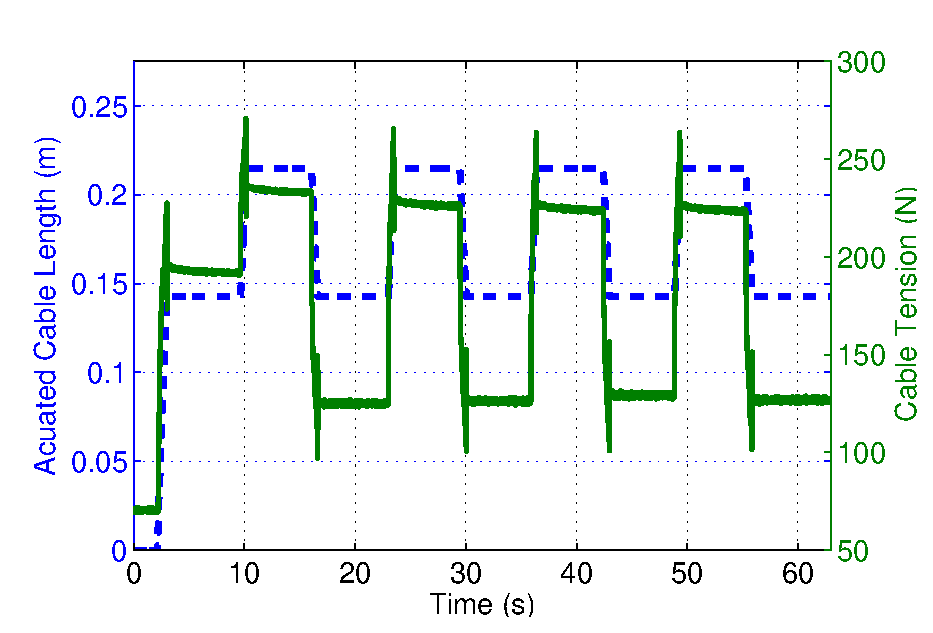
\includegraphics[width=0.8\columnwidth]{tex/img/ICRA2015_dynamic_sensor_test}
      \caption{Motor mount torque sensor data and motor position data recorded during a square wave input position trajectory for a single motor. This plot shows measured tension from the sensor and cable length from motor encoder measurements as a function of time for this dynamic movement.}
      \label{fig:sensor1data}
\end{figure}

This test was performed to demonstrate the force sensors' ability to capture data under dynamic motion.
Figure~\ref{fig:sensor1data} shows a plot of sensor data from one end cap whose motor is commanded in a square-wave position trajectory.
The position trajectory had a period of \SI{13}{\second}, and oscillated between \SI{10}{\radian} and \SI{15}{\radian} of the output shaft measured before the gearbox, by the encoder.
The trajectory of sensor torque values reasonably tracks the position square wave: the commanded position trajectory starts at 10 seconds and ends at 62 seconds, as does the sensed tension square wave.
The overshoot on the torque sensor measurements is due to the system inertia and spring dynamics.

\subsection{Global Force Redistribution Sensor Testing}

\begin{figure}[thpb]
      %\vspace{-0.5cm}
      \centering
      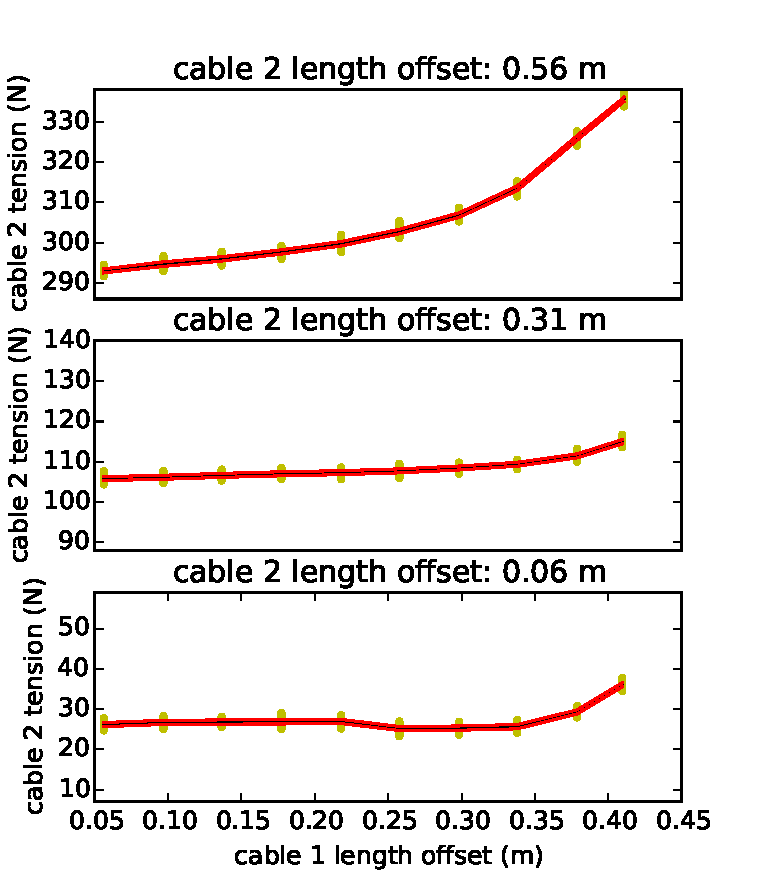
\includegraphics[width=0.55\columnwidth]{tex/img/sensor2_original}
      \caption{Global force redistribution test. Yellow marks are the means of roughly 5,000 tension sensor measurements of \emph{cable 2} opposite that which is actuated (\emph{cable 1}.) The black line shows the linear interpolation between points, with the red boundary as standard deviation. The pretension in the sensed cable is adjusted in each test, showing measurement sequences at increasing pretensions.}
      \label{fig:sensor2data_forcedistribution}
\end{figure}

A test was performed to validate the distribution of tension throughout the system, and to show that all sensors can work in conjunction simultaneously.
Figure~\ref{fig:sensor2data_forcedistribution} shows tension readings from a different motor-mount torque sensor on the opposite side of \SB{} (Cable 2) from a cable which is being retracted (Cable 1.)
Cable 2 was not actively actuated during each test.
For each plot in Figure~\ref{fig:sensor2data_forcedistribution}, the actuated cable was retracted with various step inputs marked in the figure.
Each data point in this figure (yellow) was collected by averaging data from the sensor board for a total of 5 seconds at 1 kHz, after waiting 2 seconds after the step input actuation to avoid dynamic effects.
These tests were done with different levels of pretension on the sensed cable: this pretension was adjusted by changing the length of the sensed cable.
Though the lower-pretension tests show smaller changes in readings, the higher pretensions show increasing readings which demonstrate the ability to sense forces throughout the tension network in pseudo-equilibrium states, as well as \SB{}'s passive force redistribution properties.

\subsection{Basic Locomotion}
\label{basic_locomotion}
Using a basic step input to a single motor, \SB{} can perform a simple transition from one face of the icosahedron to another.
Figure \ref{fig:superball_flop_flat} shows an test where a motor retracts a cable, induing a flop.
The idea of this type of simple transition is to deform the base equilateral triangle such that the center of mass "moves" over the triangle's edge.
The robot becomes unstable and gravity pulls the system over.
The momentum of the system then rolls the robot through the adjacent isosceles triangle to the next equilateral triangle.
In this test, the motor retraction was preset and experimentally derived earlier.

\begin{figure}[t]
    \centering
    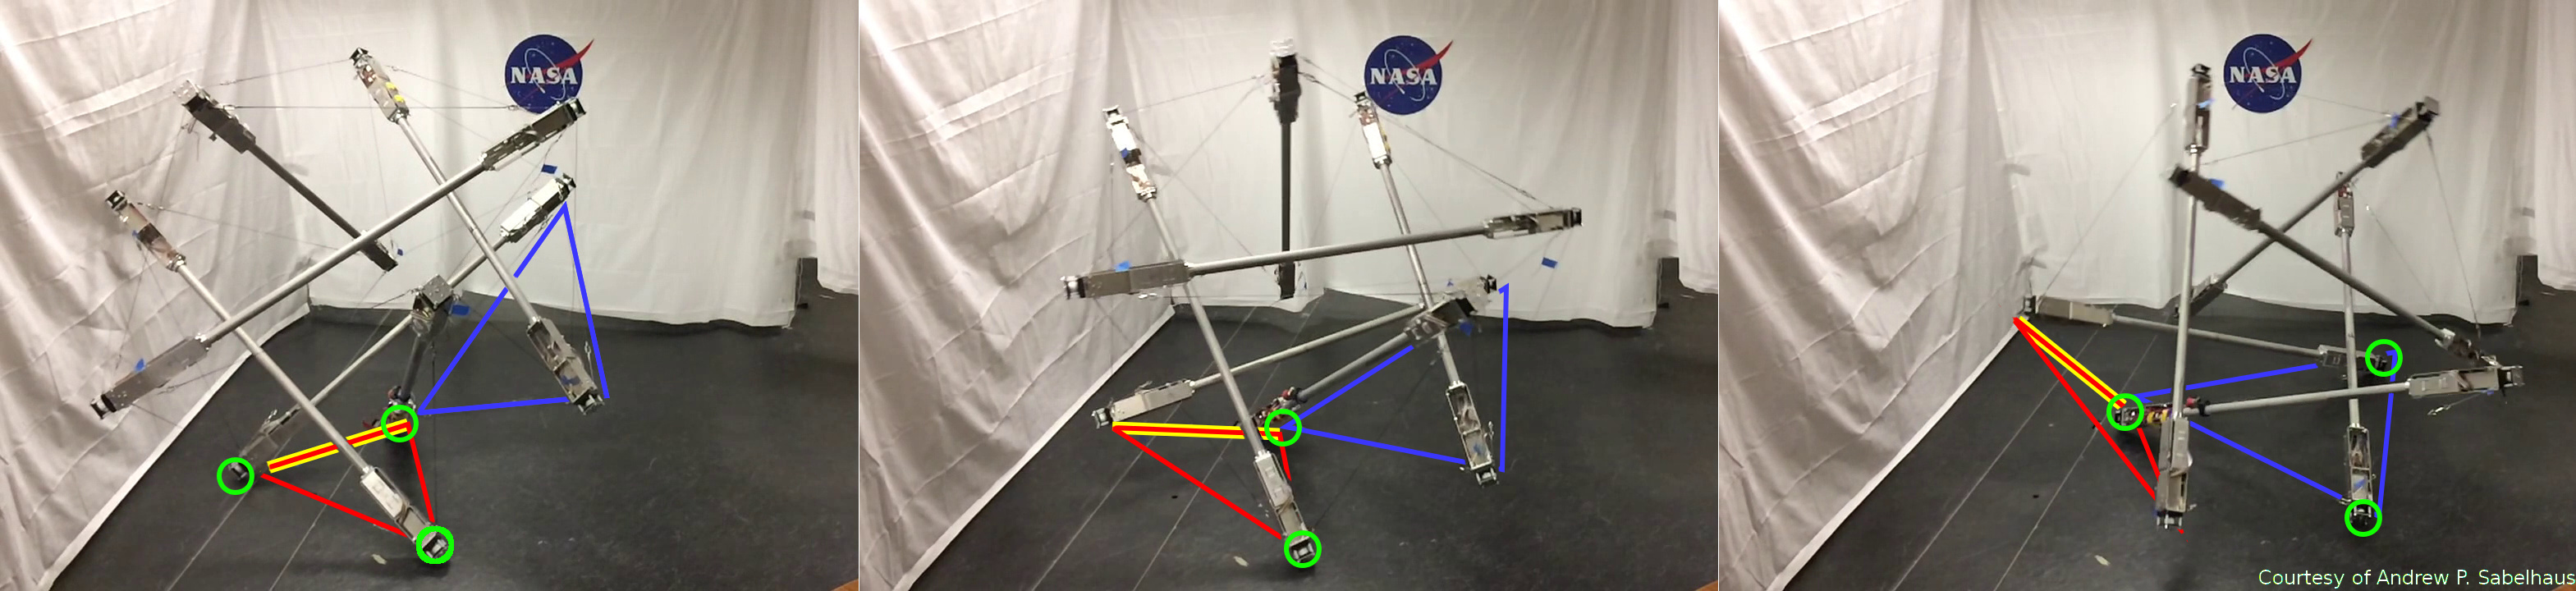
\includegraphics[width=1\linewidth]{tex/img/superball_flop_combined_betterlabels}
    \caption{\SB{} performing a single face-change movement, from one equilateral triangular face to another. The robot begins with all MTRs of the red triangle touching the ground. Then, \SB{} retracts the yellow-highlighted cable on the red triangle, inducing movement. Frame 2 shows \SB{} halfway through the movement with only two points of contact on the ground. Finally, frame 3 shows \SB{} at the end, with all 3 points of the blue triangle in ground contact.}
    \label{fig:superball_flop_flat}
\end{figure}

\section{Future Work}

%\subsection{Proposed Controls Methods}

\subsection{Open Loop Locomotion Control}
\label{open_loop}
For clarity, open loop used here is open in regards to the locomotion system's ability to change robotic motor inputs based on environmental sensing.
Work presented in~\cite{iscen2014flop} shows through simulation that a tensegrity system like \SB{} can achieve a rolling gait by deforming the triangle currently in contact with the ground.
Though \SB{} is not fully actuated (all 24 external cables are attached to motors), a derivative of this work may be able to be applied to \SB{}.
Leveraging the experimental results from section \ref{basic_locomotion}, \SB{} can achieve open loop locomotion quite easily with the addition of detecting which face of the robot is on the ground.
To achieve this ground detection, I propose to use the IMU modules on each sensor board to detect earth's gravity field and/or ground contacts when a rod contacts the ground.
Using a basic machine learning technique, like k-nearest neighbor, may enable successful classification of where the ground is in relation to the robot.

\subsection{Closed Loop Locomotion Control}
There has been preliminary results done by~\cite{burms2015online} which demonstrates a tensegrity robot sensing different enviromental terrains.
This shows promise that a tensegrity robot may sense changes in terrain without the need for extra sensors.
If a similar technique can be achieved on \SB{} in a real-time manor, then the open loop gait pattern used from \ref{open_loop} can be altered to better locomote over the sensed terrain.
This new locomotion gait may either be hand tuned parameters or learned behavior.

